\scanpage{11}
\[
 \unsure{=|\Rightarrow}
\]
\[
 \begin{aligned}
 \mathbb{P}(X)&\qquad
 P(X\times\unsure{Z|2})\overset{?}{\simeq}
 \operatorname{Hom}(\underset{\unsure{\cdot}}{\deleted{\unsure{e|\mathcal E}}Z}\times X,\mathscr E)\\
 &\qquad\mathrel{/\!/}\quad
 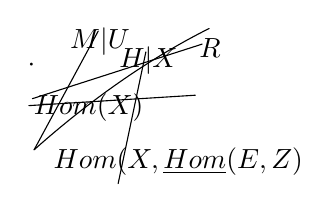
\begin{tikzpicture}[x=.011cm,y=-.011cm,baseline=(live.base),line cap=round,line join=round]
 % The cancellation paths are drawn explicitly. Invisible deleted copies retain the deletion annotation.
 \node[anchor=base west,inner sep=0] at (74,110)
 {\rlap{$\operatorname{Hom}(X)$}\phantom{$\deleted{\operatorname{Hom}(X)}$}};
 \node[inner sep=0] at (151,26)
 {\rlap{$\unsure{M|U}$}\phantom{$\deleted{\unsure{M|U}}$}};
 \node[inner sep=0] at (207,48)
 {\rlap{$\unsure{H|X}$}\phantom{$\deleted{\unsure{H|X}}$}};
 \node[inner sep=0] at (278,34)
 {\rlap{$R$}\phantom{$\deleted{R}$}};
 \draw (69,100) -- (261,88);
 \draw (73,92) -- (269,29);
 \draw (75,151) -- (149,14);
 \draw (75,151) .. controls (120,111) and (191,54) .. (277,11);
 \draw (172,190) -- (204,38);
 \node[inner sep=0] at (72,54) {$\unsure{\cdot}$};
 \node[anchor=base west,inner sep=0] (live) at (97,173)
 {$\operatorname{Hom}(X,\underline{\operatorname{Hom}}(\mathscr E,Z)$};
 \end{tikzpicture}\\
 \unsure{O|0}\subset\mathbb{P}(X)&\qquad
 \operatorname{Hom}(\mathscr E,\underline{\operatorname{Hom}}(X,Z))\\
 &\qquad\mathrel{/\!/}\\
 &\qquad P(\operatorname{Hom}(X,Z)
 \end{aligned}
\]
\figure{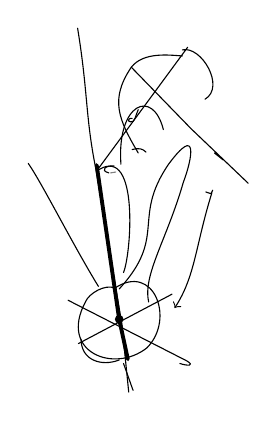
\begin{tikzpicture}[x=.011cm,y=-.011cm,line cap=round,line join=round]
% crop-candidate: scan 11
% Coordinate origin for the checked paths is approximately full scan (250,160).
\draw (63,1) .. controls (75,74) and (72,104) .. (84,163) -- (114,342) -- (122,421);
\draw[line width=1.4pt] (85,159) -- (111,337) -- (121,383);
\draw (6,157) .. controls (22,180) and (57,250) .. (87,299);
\draw (64,365) -- (172,308);
\draw (52,315) -- (189,385) .. controls (199,391) and (190,391) .. (181,388);
\draw (106,301) .. controls (151,271) and (176,337) .. (143,370)
 .. controls (105,400) and (41,375) .. (72,317) .. controls (76,307) and (95,296) .. (106,301);
\draw (67,360) .. controls (67,384) and (90,392) .. (111,384);
\fill (111,337) circle (5);
\draw (87,163) -- (190,23) (184,26) .. controls (206,21) and (234,69) .. (210,83)
 (125,46) -- (194,117) -- (260,180) (231,153) -- (221,145);
\draw (133,145) .. controls (110,106) and (100,83) .. (125,46) .. controls (139,28) and (169,32) .. (184,33);
\draw (113,158) .. controls (108,87) and (150,70) .. (162,118);
\draw (88,164) .. controls (134,137) and (125,261) .. (116,283);
\draw (111,302) .. controls (167,241) and (125,221) .. (168,158)
 .. controls (202,112) and (196,150) .. (185,179) .. controls (166,245) and (138,286) .. (145,317);
\draw[->] (218,191) .. controls (199,252) and (199,287) .. (175,324);
% Local hooks and short detached strokes: visible shapes, with no supplied letter or mathematical role.
\draw (133,95) .. controls (130,101) and (129,111) .. (124,109)
 .. controls (120,109) and (122,104) .. (126,105);
\draw (126,141) .. controls (134,139) and (138,140) .. (142,144);
\draw (105,160) .. controls (96,159) and (88,165) .. (99,168);
\draw[gray] (101,168) -- (107,167);
\draw (211,190) -- (217,192) -- (219,188);
\draw (116,388) -- (127,419);
\end{tikzpicture}}
\[
 \begin{aligned}
 \underline{\operatorname{Hom}}(X,Y)&\subset P(X\times Y)\\
 \operatorname{Hom}(\begin{tikzpicture}[baseline=(z.base),line cap=round,line join=round]
 \node[inner sep=0] (z) at (0,0) {$\deleted{\unsure{t|1}}Z$};
 \node[inner sep=0] at (.17,.48) {\unsure{\begin{tikzpicture}[line cap=round,line join=round]
 \draw (0,0) -- (.08,.06) -- (.15,.03) -- (.23,.06) -- (.30,.04);
 \fill (.38,.04) circle (.012);
 \fill[gray] (.43,.03) circle (.009);
 \end{tikzpicture}}};
 \end{tikzpicture}\times X,Y)&\subset P(Z\times X\times Y)
 \end{aligned}
\]
\diagram{\begin{tikzcd}[ampersand replacement=\&,row sep=small,column sep=small]
 \& {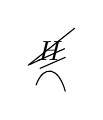
\begin{tikzpicture}[baseline=(h.base),line cap=round,line join=round]
 \node[inner sep=0] (h) at (0,0)
 {\rlap{$H$}\phantom{$\deleted{H}$}};
 \draw (-.28,-.18) -- (.31,.29);
 \draw (-.26,-.17) -- (.18,.03);
 \draw (-.13,-.22) -- (.19,-.08);
 \draw (-.18,-.43) .. controls (-.08,-.16) and (.11,-.21) .. (.19,-.51);
 \end{tikzpicture}} \& \& \\
 \& \deleted{\unsure{H|R}}P\deleted{e}\times X\times Y
       \arrow[d,"{
\begin{tikzpicture}[baseline=(u.base),line cap=round]
       \node[inner sep=0] (u) at (0,0)
       {\rlap{$\unsure{H|U}$}\phantom{$\deleted{\unsure{H|U}}$}};
       \draw (-.21,-.21) -- (.24,.36);
       \node at (.38,-.06) {$\unsure{\cdot}$};
       \end{tikzpicture}}"'] \& \& {\supset}\deleted{H}\Gamma\arrow[dll] \\
 \& P\times X\arrow[dl] \& \& U\times_{\unsure{Y|V}}U\\
 {\begin{tikzpicture}[baseline=(p.base),line cap=round]
 \node[inner sep=0] (p) at (.29,-.25) {$P$};
 \node[inner sep=0] at (-1.03,.91) {$\unsure{\cdot}$};
 \draw[gray] (-1.11,.94) .. controls (-1.10,.92) and (-1.08,.91) .. (-1.07,.90);
 \draw (-.08,1.0) .. controls (-.06,.35) and (-.12,-.55) .. (-.09,-1.04);
 \draw (-.06,.05) .. controls (-.03,-.28) and (.02,-.67) .. (.08,-.92);
 \end{tikzpicture}}
 \& \unsure{V|W}\arrow[dr,dash,shorten <=4pt,shorten >=5pt] \& \& U\arrow[ll]\arrow[dl,dash,shorten <=4pt,shorten >=5pt]\\
 \& \& P \&
\end{tikzcd}}
\figure{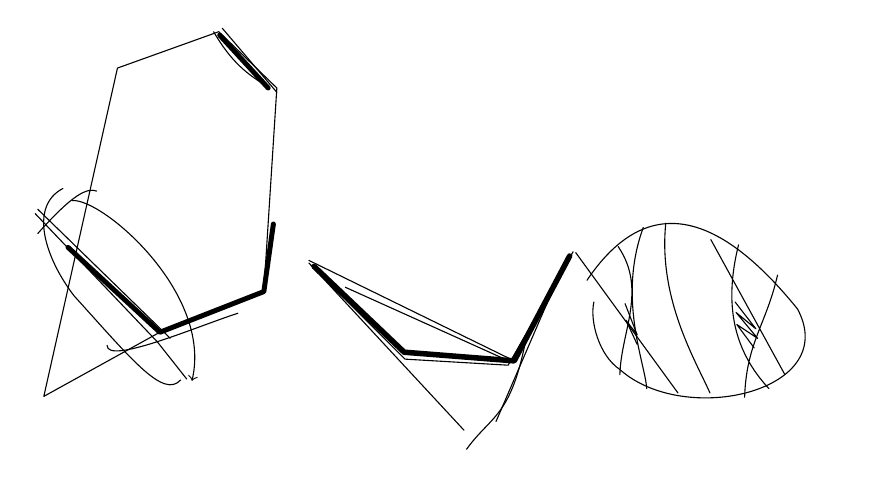
\begin{tikzpicture}[x=.011cm,y=-.011cm,line join=round,line cap=round]
% crop-candidate: scan 11
% The three bottom drawings were checked individually on the supplied halves.
\draw (13,425) -- (98,46) -- (215,4) -- (282,69) -- (267,303) -- (145,352) -- cycle;
\draw[line width=1.8pt] (216,8) -- (272,69) (278,226) -- (267,304) -- (147,351) -- (41,253);
\draw (209,4) .. controls (230,40) and (248,53) .. (272,68) (282,74) -- (219,0);
\draw (6,237) .. controls (47,191) and (63,184) .. (74,188)
 (3,214) -- (144,362) -- (178,405) (6,209) -- (159,358);
\draw (35,185) .. controls (-5,206) and (15,266) .. (48,309)
 .. controls (115,383) and (151,428) .. (171,406);
\draw[->] (46,199) .. controls (80,196) and (208,305) .. (184,407);
\draw (86,366) .. controls (86,389) and (188,345) .. (237,329);
\draw (319,271) -- (430,382) -- (549,389) -- (624,258) (319,271) -- (498,464) (535,454) -- (617,264);
\draw[line width=2pt] (325,275) -- (429,374) -- (556,384) -- (620,263);
\draw (319,268) -- (556,384) (361,299) -- (543,381);
\draw (501,486) .. controls (530,446) and (552,450) .. (570,357);
\draw (627,259) -- (745,421);
\draw (640,291) .. controls (722,169) and (814,239) .. (883,324)
 .. controls (934,419) and (753,461) .. (678,394) .. controls (654,378) and (643,338) .. (648,316);
\draw (676,252) .. controls (710,302) and (679,351) .. (678,400)
 (705,230) .. controls (675,312) and (707,386) .. (709,416)
 (731,225) .. controls (722,312) and (765,383) .. (782,421);
\draw (783,244) -- (868,399) (815,250) .. controls (797,322) and (811,374) .. (850,416)
 (860,285) .. controls (847,342) and (824,363) .. (822,426);
\draw (684,318) -- (698,354) -- (685,337) -- (698,365)
 (811,316) -- (835,347) -- (812,328) -- (837,358) -- (813,342) -- (833,369);
\end{tikzpicture}}
% archive sheet number: 10
